%%%%%%%%%%%%%%%%%%%%%%%%%%%%%%%%%%%%%%%%%
% Beamer Presentation
% LaTeX Template
% Version 1.0 (10/11/12)
%
% This template has been downloaded from:
% http://www.LaTeXTemplates.com
%
% License:
% CC BY-NC-SA 3.0 (http://creativecommons.org/licenses/by-nc-sa/3.0/)
%
%%%%%%%%%%%%%%%%%%%%%%%%%%%%%%%%%%%%%%%%%

%----------------------------------------------------------------------------------------
%	PACKAGES AND THEMES
%----------------------------------------------------------------------------------------

\documentclass{beamer}

\mode<presentation> {

% The Beamer class comes with a number of default slide themes
% which change the colors and layouts of slides. Below this is a list
% of all the themes, uncomment each in turn to see what they look like.

%\usetheme{default}
%\usetheme{AnnArbor}
%\usetheme{Antibes}
%\usetheme{Bergen}
%\usetheme{Berkeley}
%\usetheme{Berlin}
%\usetheme{Boadilla}
%\usetheme{CambridgeUS}
%\usetheme{Copenhagen}
%\usetheme{Darmstadt}
%\usetheme{Dresden}
%\usetheme{Frankfurt}
%\usetheme{Goettingen}
%\usetheme{Hannover}
%\usetheme{Ilmenau}
%\usetheme{JuanLesPins}
%\usetheme{Luebeck}
\usetheme{Madrid}
%\usetheme{Malmoe}
%\usetheme{Marburg}
%\usetheme{Montpellier}
%\usetheme{PaloAlto}
%\usetheme{Pittsburgh}
%\usetheme{Rochester}
%\usetheme{Singapore}
%\usetheme{Szeged}
%\usetheme{Warsaw}

% As well as themes, the Beamer class has a number of color themes
% for any slide theme. Uncomment each of these in turn to see how it
% changes the colors of your current slide theme.

%\usecolortheme{albatross}
%\usecolortheme{beaver}
%\usecolortheme{beetle}
%\usecolortheme{crane}
%\usecolortheme{dolphin}
%\usecolortheme{dove}
%\usecolortheme{fly}
%\usecolortheme{lily}
%\usecolortheme{orchid}
%\usecolortheme{rose}
%\usecolortheme{seagull}
%\usecolortheme{seahorse}
%\usecolortheme{whale}
%\usecolortheme{wolverine}

%\setbeamertemplate{footline} % To remove the footer line in all slides uncomment this line
%\setbeamertemplate{footline}[page number] % To replace the footer line in all slides with a simple slide count uncomment this line

%\setbeamertemplate{navigation symbols}{} % To remove the navigation symbols from the bottom of all slides uncomment this line
}

\usepackage{graphicx} % Allows including images
\usepackage{subcaption}
\usepackage{booktabs} % Allows the use of \toprule, \midrule and \bottomrule in tables
\usepackage{amsmath}
\usepackage{tikz}
\usepackage{csvsimple}
\usepackage[
  backend=biber,
  style=apa,
  citestyle=apa
]{biblatex}
\usetikzlibrary{arrows}

\addbibresource{references.bib}

\def\indep{\perp \!\!\! \perp}

%----------------------------------------------------------------------------------------
%	TITLE PAGE
%----------------------------------------------------------------------------------------

\title[Causal Discovery DSGE]{Causal Discovery of DSGE Models} % The short title appears at the bottom of every slide, the full title is only on the title page

\author{Emmet Hall-Hoffarth} % Your name
\institute[Oxford] % Your institution as it will appear on the bottom of every slide, may be shorthand to save space
{
University of Oxford \\ % Your institution for the title page
\medskip
\textit{emmet.hall-hoffarth@economics.ox.ac.uk} % Your email address
}
\date{\today} % Date, can be changed to a custom date

\begin{document}

\begin{frame}
    \titlepage % Print the title page as the first slide
\end{frame}

\begin{frame}
    \frametitle{Overview} % Table of contents slide, comment this block out to remove it
    \tableofcontents % Throughout your presentation, if you choose to use \section{} and \subsection{} commands, these will automatically be printed on this slide as an overview of your presentation
\end{frame}

\section{Introduction}

\begin{frame}
    \frametitle{Introduction}
    \begin{itemize}
        \item I develop an algorithm for agnostic and data-driven causal discovery of a unique state-space model and associated family of DSGE models which are \textit{valid} (in a sense that I shall make specific later) relative to some observational data.
        \item I provide proof that the solution to this procedure is asymptotically unique and consistent, along with empirical evidence that it performs well with realistic sample sizes.
    \end{itemize}
\end{frame}

\section{What?}

\begin{frame}
    \centering
    \huge
    What does this mean?
\end{frame}

\begin{frame}
    \frametitle{Causal Discovery}
    \begin{itemize}
        \item \textit{Causal Discovery} is a field initiated by the work of Pearl, Spirtes, and others involving using large data sets and algorithms to develop models that can make counterfactual predictions.
        \item One approach to this involves graphical models such as directed acyclical graphs (DAGs).
        \item Algorithms seek to identify a DAG from data using either a score-based (likelihood maximisation) or constraint-based (conditional independence testing) approach.
        \item \citeauthor{imbens2019potential} (\citeyear{imbens2019potential}) calls for more applications of graphical models to be demonstrated within the field of economics.
    \end{itemize}
\end{frame}

\begin{frame}
    \frametitle{DSGE Models}
    \begin{minipage}{0.4\textwidth}
        \centering
        Consumer problem
        \begin{align*}
            & \max \text{ } \sum_{t=0}^{\infty} \beta^t U(C_t, L_t, ...) \text{ } s.t. \\
            & \text{ } P_t C_t + ... \leq W_t L_t + ... \text{ } \forall t \\
            & \lim_{T \rightarrow \infty} \beta^T \lambda_{x,T} x_T \rightarrow 0 \text{ } \forall x \in \{K, B, ...\}
        \end{align*}
    \end{minipage}
    \begin{minipage}{0.4\textwidth}
        \centering
        Firm problem
        \begin{align*}
            \max \text{ } & P_t f(L_t, ...) - W_t L_t \text{ } \forall t \\
        \end{align*}
    \end{minipage}
    \centering
    Competitive equilibrium, market clearing conditions ...
\end{frame}

\begin{frame}
    \frametitle{State Space Representation}
    \begin{itemize}
        \item Solve out these equations and take a log-linear approximation to the model that takes on the following general form: 
    \end{itemize}
        \begin{align}
            \vec{y}_t &= \vec{A} \vec{x}_{t-1} + \vec{B} \vec{z}_{t} \label{ss_solution:x}\\
            \vec{x}_t &= \vec{C} \vec{x}_{t-1} + \vec{D} \vec{z}_{t} \label{ss_solution:y}\\
            \vec{z}_t &= \vec{E} \vec{z}_{t-1} + \vec{\epsilon}_{t} \label{ss_solution:z}
        \end{align}
    \begin{itemize}
        \item This is a partition of the variables $\vec{w}_t$ in the model into three categories:
        \begin{itemize}
            \item $\vec{x}_t$: predetermined or endogenous state variables
            \item $\vec{y}_t$: control variables or "jumpers"
            \item $\vec{z}_t$: exogenous state variables
        \end{itemize}
        \item The algorithm identifies this partition (and the matrices $\vec{A}$ - $\vec{E}$).
    \end{itemize}
\end{frame}

\section{Why?}

\begin{frame}
    \centering
    \huge
    Why is this useful?
\end{frame}

\begin{frame}
    \frametitle{Reduction of problem space}
    \begin{itemize}
        \item Given a set of observations over $k$ variables there are $3^k$ possible state space representations.
        \begin{itemize}
            \item Choice of model is \textit{trinomial}
        \end{itemize}
        \item Reducing this to just one is then a huge reduction in the space of models that need to be considered.
        \item Note that this does not mean that we identify a unique DSGE model --- different microfoundations may give rise to the same state space representation.
    \end{itemize}
\end{frame}

\begin{frame}
    \frametitle{Agnosticism}
    \begin{itemize}
        \item Assumptions we use are very minimal:
        \begin{itemize}
            \item The true DGP of the macroeconomy can be modelled as some sort of log-linear DSGE model.
            \item \textit{Casual Markov Assumption} --- All variables are independent of their non-descendants given their parents \parencite{spirtes2016causal}.
            \begin{itemize}
                \item This is the statement that causality is equivalent to conditional independence (as implied by a DAG).
                \item DSGE models have this property. So while in general this is a separate assumption it is in this case implied by the first condition.
            \end{itemize}
            \item \textit{Faithfulness} --- observed conditional indepedence are real features of the DGP. Effects do not cancel out exactly.
            \item Linearity, Gaussian shocks --- these can be relaxed.
        \end{itemize}
        \item As a result the solution produced reflects the data to the greatest extent possible.
    \end{itemize}
\end{frame}

\begin{frame}
    \frametitle{Inference}
    \begin{itemize}
        \item We cannot pin down a unique DSGE microfoundation given its state space form. However, we can make statements about certain kinds of assumptions.
        \item For example, if we find that consumption is predetermined, this is evidence that any sensible model should include habits in consumption (although you could come up with some other explanation).
        \item If we find that inflation is a endogenous state then we have evidence of persistence in inflation, which might be explained by for example indexing. If it is a control we have evidence that inflation is strictly forward-looking.
        \item These types of inferences are particularly meaningful in the context of the previous slide.
    \end{itemize}
\end{frame}

\section{How?}
\begin{frame}
    \centering
    \huge
    How is this even possible?
\end{frame}

\begin{frame}
    \frametitle{DAGs}
    \begin{itemize}
        \item We can represent the state space representation as a DAG.
    \end{itemize}
    \begin{figure}
        \centering
        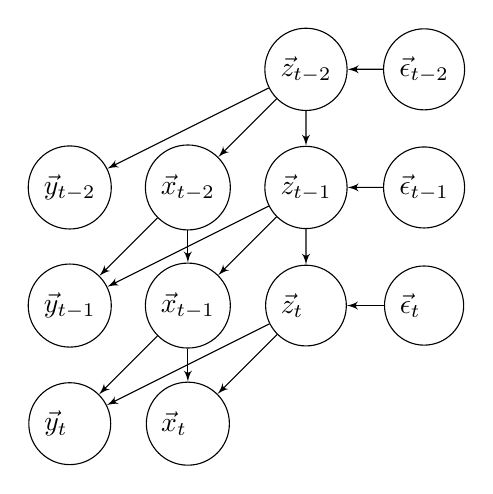
\begin{tikzpicture}[scale=1.5]
          \tikzset{
            vertex/.style={circle,draw, minimum size=2em},
            edge/.style={->,> = latex'}
          }
          % vertices
          \node[vertex] (zt) at (1 ,0) {$\vec{z}_{t\quad}$};
          \node[vertex] (zt1) at (1 , 1) {$\vec{z}_{t-1}$};
          \node[vertex] (zt2) at (1 , 2) {$\vec{z}_{t-2}$};
          \node[vertex] (xt) at (0 ,-1) {$\vec{x}_{t\quad}$};
          \node[vertex] (xt1) at (0 , 0) {$\vec{x}_{t-1}$};
          \node[vertex] (xt2) at (0 , 1) {$\vec{x}_{t-2}$};
          \node[vertex] (yt) at (-1,-1) {$\vec{y}_{t\quad}$};
          \node[vertex] (yt1) at (-1, 0) {$\vec{y}_{t-1}$};
          \node[vertex] (yt2) at (-1, 1) {$\vec{y}_{t-2}$};
          \node[vertex] (et) at (2 , 0) {$\vec{\epsilon}_{t\quad}$};
          \node[vertex] (et1) at (2 , 1) {$\vec{\epsilon}_{t-1}$};
          \node[vertex] (et2) at (2 , 2) {$\vec{\epsilon}_{t-2}$};
      
          %edges
          \draw[edge] (et) -- (zt);
          \draw[edge] (et1) -- (zt1);
          \draw[edge] (et2) -- (zt2);
          \draw[edge] (zt2) -- (zt1);
          \draw[edge] (zt1) -- (zt);
          \draw[edge] (xt2) -- (xt1);
          \draw[edge] (xt1) -- (xt);
          \draw[edge] (zt2) -- (xt2);
          \draw[edge] (zt1) -- (xt1);
          \draw[edge] (zt) -- (xt);
          \draw[edge] (zt2) -- (yt2);
          \draw[edge] (zt1) -- (yt1);
          \draw[edge] (zt) -- (yt);
          \draw[edge] (xt2) -- (yt1);
          \draw[edge] (xt1) -- (yt);
        \end{tikzpicture}
      \end{figure}
\end{frame}

\begin{frame}
    \frametitle{(Aside) Is this sensible?}
    \centering
    \begin{minipage}{0.4\textwidth}
        \begin{figure}
            \centering
            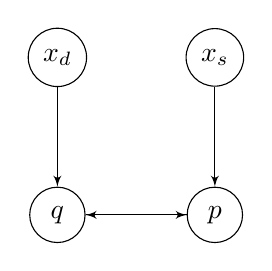
\begin{tikzpicture}[scale=2]
            \tikzset{
                vertex/.style={circle,draw, minimum size=2em},
                edge/.style={->,> = latex'}
            }
            % vertices
            \node[vertex] (q) at (0,0) {$q$};
            \node[vertex] (p) at (1,0) {$p$};
            \node[vertex] (xd) at (0,1) {$x_d$};
            \node[vertex] (xs) at (1,1) {$x_s$};
        
            %edges
            \draw[edge] (q) -- (p);
            \draw[edge] (p) -- (q);
            \draw[edge] (xd) -- (q);
            \draw[edge] (xs) -- (p);
            \end{tikzpicture}
        \end{figure}
        \small
        \begin{align*}
            p = \alpha_p + \beta_{ps} x(s) + \beta_{pq} q + \epsilon_{p} \\
            q = \alpha_q + \beta_{qd} x(d) + \beta_{qp} p + \epsilon_{q}
        \end{align*}
    \end{minipage}
    %
    \begin{minipage}{0.05\textwidth}
        \centering
        $\iff$
    \end{minipage}
    %
    \begin{minipage}{0.4\textwidth}
        \begin{figure}
            \centering
            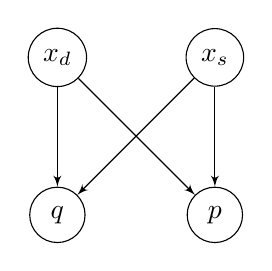
\begin{tikzpicture}[scale=2]
            \tikzset{
                vertex/.style={circle,draw, minimum size=2em},
                edge/.style={->,> = latex'}
            }
            % vertices
            \node[vertex] (q) at (0,0) {$q$};
            \node[vertex] (p) at (1,0) {$p$};
            \node[vertex] (xd) at (0,1) {$x_d$};
            \node[vertex] (xs) at (1,1) {$x_s$};
        
            %edges
            \draw[edge] (xd) -- (p);
            \draw[edge] (xd) -- (q);
            \draw[edge] (xs) -- (q);
            \draw[edge] (xs) -- (p);
            \end{tikzpicture}        
        \end{figure}
        \tiny
        \begin{align*}
            p = \frac{1}{1-\beta_{pq}\beta_{qp}}[& (\alpha_p + \beta_{pq} \alpha_q) + \beta_{ps} x(s) + \\ & \beta_{pq} \beta_{qd} x(d) + (\epsilon_p + \beta_{pq} \epsilon_q)] \\
            q = \frac{1}{1-\beta_{qp}\beta_{pq}}[& (\alpha_q + \beta_{qp} \alpha_p) + \beta_{qd} x(d) + \\ & \beta_{qp} \beta_{ps} x(s) + (\epsilon_q + \beta_{qp} \epsilon_p)]
        \end{align*}
    \end{minipage}
    \begin{itemize}
        \item Understanding response to shocks does not require inference of "deep" parameters ($\beta_{xy}$).
    \end{itemize}
\end{frame}

\begin{frame}
    \frametitle{Conditional Independence (I)}
    \begin{itemize}
        \item Given the Causal Markov assumption we can infer the following relationships from this DAG: 
    \end{itemize}
    \begin{align}
        x_t \indep x^{\prime}_{t} \,||\,& [\vec{x}_{t-1},\vec{z}_t] \text{ for all } (x_t, x^{\prime}_{t}) \in [\vec{x}_t, \vec{y}_t] \label{constraint_test:1} \\
        x_{t-1} \indep z_{t} \,||\,& \vec{z}_{t-1} \text{ for all } x_{t-1} \in \vec{x}_{t-1} \text{ and } z_{t} \in \vec{z}_t \label{constraint_test:3} \\
        x_t \indep z_{t-1} \,||\,& [\vec{x}_{t-1}, \vec{z}_t] \text{ for all } x_t \in [\vec{x}_t, \vec{y}_t] \text{ and } z_{t-1} \in \vec{z}_{t-1} \label{constraint_test:2} \\
        z_t \indep z^{\prime}_{t} || \vec{z}_{t-1} & \text{ for all } z_t \not = z^{\prime}_{t} \in \vec{z}_t \label{constraint_test:4}
      \end{align}
    \begin{itemize}
        \item In the paper I show that under the stated assumptions if all conditional independence relationships are known there is exactly one state-space model that satisfies (\ref{constraint_test:1}), (\ref{constraint_test:3}) and the minimum state variable criterion (MSV) \parencite{mccallum1999role}. I refer to the satisfaction of these criteria as \textit{validity}.
    \end{itemize}
\end{frame}

\begin{frame}
    \frametitle{Conditional Independence (II)}
    \begin{itemize}
        \item In reality conditional independence is not known, so we implement a feasible test.
        \item Given that we are dealing with Gaussian variables independence is equivalent to zero correlation/covariance, and likewise conditional independence is equivalent to zero correlation/covariance between residuals, having partialed out the conditioning set.
        \item With some slight modification all 4 conditions can be combined into a single test on a covariance matrix.
        \item In particular, test whether $\vec{x}_{t-1}$, $\vec{y}_{t-1}$, $\vec{z}_{t}$, and (optionally) $\vec{z}_{t-2}$ are \textit{completely independent} (covariance matrix is diagonal), conditional on $\vec{x}_{t-2}$ and $\vec{z}_{t-1}$.
        \item Many statistical tests are available for this purpose, I implement one found in \parencite{srivastava2005some}.
    \end{itemize}
\end{frame}

\begin{frame}
    \frametitle{Scoring}
    \begin{itemize}
        \item In finite samples, it is not uncommon to find that more than one model is \textit{valid}, however, it is usually a small number compared to the search space.
        \item In order to differentiate between this valid models I maximise a score function, which in most cases is the likelihood function of the model. I also implement penalised scores (AIC/BIC), but these are less useful because the models that survive the CI testing tend to have very similar structures/complexity.
        \item In general, one can just maximise the score function over the set of all models, however, I argue against this approach because it is not necessarily the case that the model with the best predictive accuracy gives the most reasonable causal explanation.
    \end{itemize}
\end{frame}

\begin{frame}
    \frametitle{Algorithm}
    \begin{itemize}
        \item To find the valid model(s), iterate over all possible models and apply the test (brute force).
        \item We can make this less onerous by applying MSV and stopping once we have found a valid model.
        \item If we find more than one valid model choose a winner using the score function.
        \item This algorithm will consistently identify the unique valid model as $n \rightarrow \infty$ with the number of variables fixed because the power of the CI test to reject incorrect models goes to 1.
        \begin{itemize}
            \item We will still have a significance level $\alpha$ probability of rejecting the correct model, and thus finding no solution in the asymptotic case.
            \item To counter this we can lower $\alpha$ as $n$ increases. 
            \item $\alpha$ is the only tuning parameter of this algorithm.
        \end{itemize}
    \end{itemize}
\end{frame}

\begin{frame}
    \frametitle{Results (I)}
    \begin{itemize}
        \item Baseline RBC model.
        \item 9 Observables, true partition is $\vec{z} = [g \text{ } z]$, $\vec{x} = [k]$, $\vec{y} = [y \text{ } c \text{ } i \text{ } r \text{ } w \text{ } l]$.
        \item With full sample of $10^5$ observations the only valid partition is the ground truth.
        \item 834 models considered (models with $1 \leq$ \# state variables $\leq 3$).
        \item 19683 possible models reduced to 1.
    \end{itemize}
\end{frame}

\begin{frame}
    \frametitle{Results (II)}
    \begin{itemize}
        \small
        \item 1000 iterations, 100 sample size
        \item Wins = number of times model selected, Valid = number of times model is valid relative to CI test
    \end{itemize}
    \begin{table}
        \centering
        \tiny
        \begin{tabular}{|c|c|c|l|l|}
            \bfseries Index & \bfseries Exogenous States & \bfseries Endogenous States & \bfseries Wins & \bfseries Valid
            \csvreader[head to column names]{./files/rbc_wins_new.csv}{}
            {\\\index & \exostates & \endostates & \wins & \valid}
        \end{tabular}
    \end{table}
\end{frame}

\section{Conclusion}

\begin{frame}
    \frametitle{Limitations}
    \begin{itemize}
        \item Does not solve microeconomic dissonance
        \begin{itemize}
            \item Researchers still need to specify a structural model if they wish to make inferences about the counterfactual effects of structural parameter changes.
        \end{itemize}
        \item Type II error can be a problem on realistic data sizes
        \begin{itemize}
            \item We rely on the rejection of incorrect models to a large degree
            \item If there are models similar to the true solution and sample sizes are small we can end up with the wrong solution.
        \end{itemize}
        \item Computational Complexity
        \begin{itemize}
            \item Considering up to $3^k$ models can become very costly as $k$ grows.
            \item It is unclear the extent to which heuristic algorithms can improve the complexity as the search space is likely quite jagged and also this would threaten the agnosticism of the algorithm which is one of its primary benefits.
        \end{itemize}
    \end{itemize}
\end{frame}

\begin{frame}
    \frametitle{Conclusion}
    \begin{itemize}
        \item I introduce a test and algorithm to identify a unique state-space model (and associated family of DSGE models) which is \textit{valid} relative to some observed data.
        \item This procedure is asymptotically consistent and empirical results show it performs well on realistic sample sizes.
        \item One approach to applying causal discovery tools in the context of economics.
    \end{itemize}
\end{frame}

\begin{frame}
    \frametitle{Citations}
    \printbibliography
\end{frame}

\end{document}